% Saved paired-root evidence; only deployable scorers are plotted.
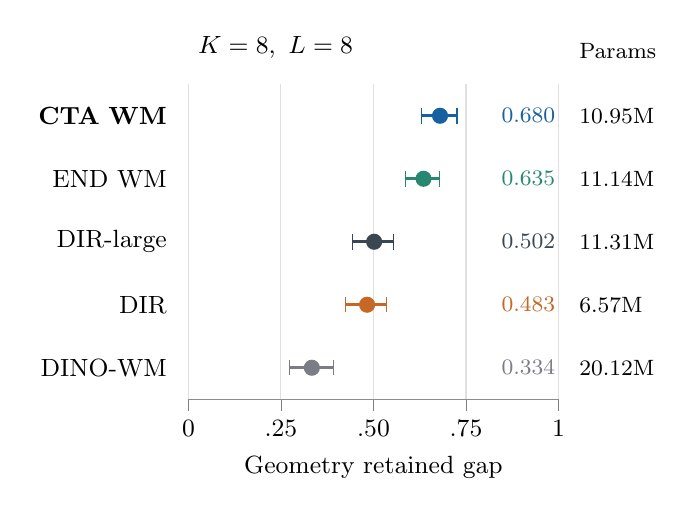
\begin{tikzpicture}
\definecolor{ctablue}{HTML}{1761A0}
\definecolor{ctagreen}{HTML}{288770}
\definecolor{ctaorange}{HTML}{C56826}
\definecolor{ctadark}{HTML}{3A4651}
\definecolor{ctagrey}{HTML}{7A7C86}
\begin{axis}[
 scale only axis,width=4.7cm,height=4.0cm,
 xmin=0,xmax=1,ymin=.5,ymax=5.5,
 xtick={0,.25,.5,.75,1},xticklabels={0,.25,.50,.75,1},
 ytick={5,4,3,2,1},yticklabels={\textbf{CTA WM},END WM,DIR-large,DIR,DINO-WM},
 font=\fontsize{9}{10}\selectfont,
 yticklabel style={text width=1.65cm,align=right},
 xlabel={Geometry retained gap},
 axis x line*=bottom,axis y line*=left,
 y axis line style={draw=none},axis line style={black!45},
 tick align=outside,ytick style={draw=none},
 xmajorgrids=true,grid style={black!12},clip=false,
]
\node[anchor=south west,font=\fontsize{9}{10}\selectfont] at (axis cs:0,5.75) {$K=8,\ L=8$};
\node[anchor=south west,font=\fontsize{8}{9}\selectfont] at (axis cs:1.03,5.75) {Params};
\addplot[only marks,mark=*,mark size=2.4pt,color=ctablue,line width=1pt,error bars/.cd,x dir=both,x explicit,error bar style={line width=1pt},error mark options={rotate=90,mark size=2.8pt}] coordinates {(0.679928144,5) +=(0.045792090,0) -=(0.050448001,0)};
\node[anchor=west,font=\fontsize{8}{9}\selectfont,text=ctablue] at (axis cs:.82,5) {0.680};
\node[anchor=west,font=\fontsize{8}{9}\selectfont] at (axis cs:1.03,5) {10.95M};
\addplot[only marks,mark=*,mark size=2.4pt,color=ctagreen,line width=1pt,error bars/.cd,x dir=both,x explicit,error bar style={line width=1pt},error mark options={rotate=90,mark size=2.8pt}] coordinates {(0.635333515,4) +=(0.042479669,0) -=(0.047753486,0)};
\node[anchor=west,font=\fontsize{8}{9}\selectfont,text=ctagreen] at (axis cs:.82,4) {0.635};
\node[anchor=west,font=\fontsize{8}{9}\selectfont] at (axis cs:1.03,4) {11.14M};
\addplot[only marks,mark=*,mark size=2.4pt,color=ctadark,line width=1pt,error bars/.cd,x dir=both,x explicit,error bar style={line width=1pt},error mark options={rotate=90,mark size=2.8pt}] coordinates {(0.501882175,3) +=(0.051130099,0) -=(0.057360646,0)};
\node[anchor=west,font=\fontsize{8}{9}\selectfont,text=ctadark] at (axis cs:.82,3) {0.502};
\node[anchor=west,font=\fontsize{8}{9}\selectfont] at (axis cs:1.03,3) {11.31M};
\addplot[only marks,mark=*,mark size=2.4pt,color=ctaorange,line width=1pt,error bars/.cd,x dir=both,x explicit,error bar style={line width=1pt},error mark options={rotate=90,mark size=2.8pt}] coordinates {(0.482833192,2) +=(0.052254867,0) -=(0.057435807,0)};
\node[anchor=west,font=\fontsize{8}{9}\selectfont,text=ctaorange] at (axis cs:.82,2) {0.483};
\node[anchor=west,font=\fontsize{8}{9}\selectfont] at (axis cs:1.03,2) {6.57M};
\addplot[only marks,mark=*,mark size=2.4pt,color=ctagrey,line width=1pt,error bars/.cd,x dir=both,x explicit,error bar style={line width=1pt},error mark options={rotate=90,mark size=2.8pt}] coordinates {(0.333532439,1) +=(0.059296528,0) -=(0.061128305,0)};
\node[anchor=west,font=\fontsize{8}{9}\selectfont,text=ctagrey] at (axis cs:.82,1) {0.334};
\node[anchor=west,font=\fontsize{8}{9}\selectfont] at (axis cs:1.03,1) {20.12M};
\end{axis}
\end{tikzpicture}
